% #############################################################################
% This is Chapter 4
% !TEX root = ../main.tex
% #############################################################################
% Change the Name of the Chapter i the following line
\fancychapter{Evaluation}
%\cleardoublepage
\label{chap:evaluation}
 
This chapter focuses on the evaluation of the proposed framework from two perspectives: in \cref{sec:qualitative}, we discuss the qualitative properties of the optimization framework, outlining the flexibility and heterogeneity of the provided algorithms, while in \Cref{sec:quantitative}, we assess the viability of the current prototype in the architectural practice by applying it to address three \ac{BPO} case studies. These optimization case studies corroborate the suitability of the algorithmic framework described in \cref{chap:implement}, by using the optimization framework and the Khepri \ac{AD} tool to enable the application of different optimization algorithms. 

Overall, this evaluation aims to answer the following questions: 
\begin{itemize}
	\item Do the studied algorithms present benefits for the architectural practice? Particularly, are they able to reduce the impact of the expensive performance analysis that are typically employed in building design?
	\item Is there any algorithm or class of algorithms that constantly outperforms others?
	% \item Is there any difference between the different \ac{MOO} approaches? \todo{PAPER ACADIA}
	\item Is the proposed framework applicable to the architectural practice? 
\end{itemize}

\section{Qualitative Evaluation}
\todo{REVER}
\label{sec:qualitative}
The quantitative evaluation of optimization frameworks involve considering multiple aspects, including the flexibility, adaptability, diversity of algorithms, ease of use, among others. Calling upon the \acp{NFLT} discussed in \Cref{ssec:comparisondfo}, some algorithms are really good solvers for some problems and very poor solvers for others~\cite{Wolpert1997NFLT}. Selecting the right algorithm can have a great impact in the efficiency of optimization processes. Particularly, in building design, to benefit from such performance gains, diversity of algorithms allows to face each problems' characteristics differently, enabling the identification of most promising algorithms. In addition to the algorithms' diversity, algorithms should be effortlessly run, without the need for many manual changes, in order to be easily used by less experienced users. Notwithstanding their innate simplicity, optimization frameworks should also be flexible enough to enable more experienced users to fine-tune them according to their expertise, thus fostering more efficient optimization processes. At last, a good framework should adapt to handle different problems.

Regarding the adaptability of the current implementation of the framework, it provides mechanisms to address both single- and multi-objective problems: 15 \ac{SOO} algorithms and 13 \acp{MOEA}, respectively. Simpler approaches, like the design of experiments approach, discussed in \cref{ssec:doe}, are also possible using one of the 5 sampling methods available in the prototype. Moreover, a crucial feature of this framework is that it provides 10 \ac{ML} algorithms to be used with other techniques, thus allowing to reduce the time complexity involved in building design. 

In \cref{chap:architecture}, \cref{table:algorithms} presents a view of the algorithms supported by the framework, discriminated by class and domain. When comparing to currently existing tools in architecture, our solution presents a more extense and diverse set of algorithms, which can be explored to address a wider variety of problems. Moreover, while the existing tools rely on a unique optimization approach (e.g., \ac{SOO}, or Pareto-based optimization), our solution adapts to the user needs, providing the necessary mechanisms to the different approaches.

Unlike existing tools, which are implemented on top of visual programming languages, like Grasshopper and Dynamo, the framework is currently implemented on top of a textual programming language. Although the graphical feel of the visual paradigm provides a more comfortable experience to less experienced users, the fact that the framework makes use of the textual paradigm confers more scalability and portability to the achieved designs, thus allowing users to seamless apply optimization to more complex buildings. To make it more appealing to less experienced users, the developed optimization framework is in a ready-to-use format, where every parameter of an optimization process is configured by default.  

Besides the ready-to-use format, the framework supports finer configurations of the different algorithms, thus allowing more experienced users to employ their knowledge to fine-tune and, if desired, to combine different algorithms. 

Moreover, given the importance of testing different algorithms before settling for a single one~\cite{Wortmann2016BBO}, the prototype provides the necessary mechanisms to facilitate and automate testing multiple algorithms with no additional efforts for the user. Conversely, existing architectural tools require the user's intervention in order to test different algorithms, either by dragging other optimizer components and making necessary changes in the design script or, when possible, by simply re-configuring the optimization tool to use one of the other supported algorithms. 

Regarding the post-processing and logging mechanisms, the proposed framework is automatically configured to produce complete log files, including all the information about the algorithms and problems being addressed, as well as a real-time log of the different solutions explored during the optimization run. This differs from existing tools, which only made the log files available in the end of the run. That being said, some of the currently existing tools still outperform the proposed prototype in terms of the visualization and interactivity features. The proposed provides visual interactive Python scripts that read the log files and produce the corresponding plots. However, these plots are not updated in real-time, instead requiring the user to re-run the script.

Finally, in order to use the optimization framework, the user only needs to create the \ac{AD} and model the corresponding optimization problem, i.e., define the variables and its bounds, the objectives, and, if necessary, the constraints. In contrast to existing architectural optimization tools, which require the modification of the optimization script (e.g., drag other components, redefine the optimization problem, change the optimization tool), our framework requires no such effort. Instead, the user only needs to specify the algorithms that he wishes to apply and configure them accordingly.

% #############################################################################
\section{Quantitative Evaluation}
\label{sec:quantitative}

In order to study and explore the effectiveness of algorithms within building design practices, we evaluate the performance of different algorithms using the optimization framework, discussed in \cref{chap:implement}. Moreover, we evaluate the real applicability of such framework in three case studies, two of which were proposed by a small-scale architectural studio\footnote{Atelier dos Remédios: http://atrem.eu/}: (1) the optimization of the lighting conditions of a solarium in a private house in Portugal; (2) the optimization of the structural behavior and the elegance of an arc-shaped space frame structure; and (3) the optimization of the cost and the lighting conditions of an exhibition room in an arts pavilion.   

In order to measure the effectiveness of the optimization algorithms, different factors must be considered: (1) the optimization time is sensitive to the computational power of the machine where the algorithm is being run, (2) the non-determinism of several optimization algorithms, and (3) the hyperparameters of optimization algorithms. Firstly, to remove the time dependency of the machine and function's complexity, we measure the performance of the optimization algorithm in terms of the number of function evaluations, which is proportional to the actual time spent by the optimization process. Secondly, the stochastic character of several optimization algorithms (e.g., random modifications of solutions, random generation of design solutions, random initial points) might yield different results even when ran twice under the same configurations. To address this limitation, we run each stochastic algorithm 3 times and we use the average of the values to draw conclusions. Finally, the algorithm's performance for each problem can be better or worse depending on its configurations. To this end, we opt for using the default algorithm's configurations, thus emulating the case when architect's knowledge does not suffice to properly fine-tune the algorithm.
 
% #############################################################################
\subsection{Ericeira House: Solarium}
The first case study involves the optimization of the lighting conditions of a room in an isolated private house in Portugal~\cite{Caetano2018,Belem2018optimizeddesign}. The room was designed with a set of façade shading panels that modulate the daylight conditions on the interior of the room. Depicted in \cref{fig:ericeira_panels_explanation}, the panels are composed of a set of horizontal wood bars of different sizes, which alternate between one full-length bar and a set of smaller bars. For aesthetics reasons, the size and position of the smaller bars along the panel's width were randomized. The final pattern of the façade's shading panels is, thus, defined in function of four variables: the length’s step, the maximum distance separating two consecutive bars, and the minimum and maximum lengths of the smaller bars. Initially, the goal was to find a solution for the shading panels that maximized the room's daylight performance, which was measured using the \ac{sUDI} metric~\cite{Nabil2006}. In general, it is known that the more openings in the shading panels, the more daylight will enter the room. However, this may also cause situations of uncomfortable glare and therefore, which must be be accounted for. Moreover, taking into account aesthetics, the architects initially imposed a few constraints on the variables to reflect their intention for more dense patterns, i.e., with less openings. \Cref{fig:ericeira_multiple_panels} represents some design variations, ranging from denser patterns, with lower \ac{sUDI} values, to sparser ones, with higher \ac{sUDI} values.

\begin{figure}[htbp]
	\centering
	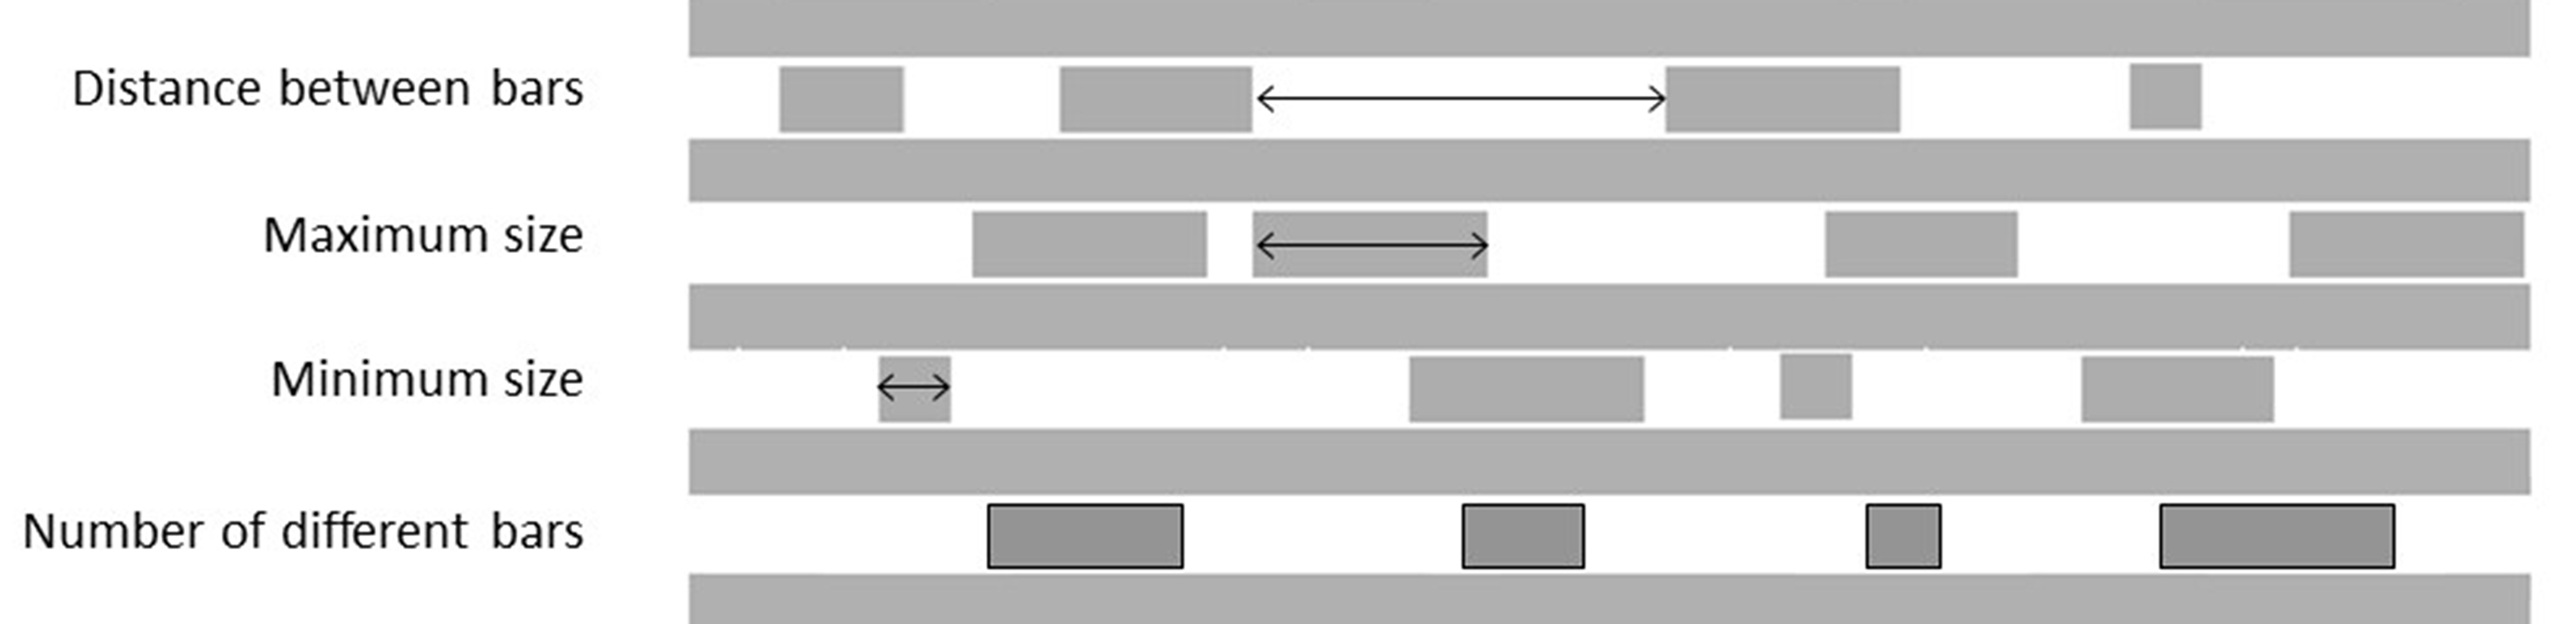
\includegraphics[width=\textwidth]{Images/Evaluation/Ericeira_1.jpg}
	\caption{Ericeira Solarium: Representation of the shading panels' geometric pattern and the patterns' design variables.}
	\label{fig:ericeira_panels_explanation}
\end{figure}

Our first approach to this case study was to a simple design of experiments \cite{Caetano2018}, where we used two sampling algorithms to generate different design approaches: the Monte Carlo sampling and the Latin hypercube sampling algorithms (see \cref{appendix:AlgorithmsDefinitions}). This approach allowed us to exploit the knowledge about the problem to produce a more efficient optimization process, by incrementally narrowing down the variables' bounds and, hence, enforcing the sampling of more efficient designs. %\Cref{fig:ericeira_doe} shows an example of the results obtained during this process, as well as the solutions that were presented to the architects, so that they would choose the one that better suited their intentions.

%\begin{figure}[htbp]
%	\centering
%	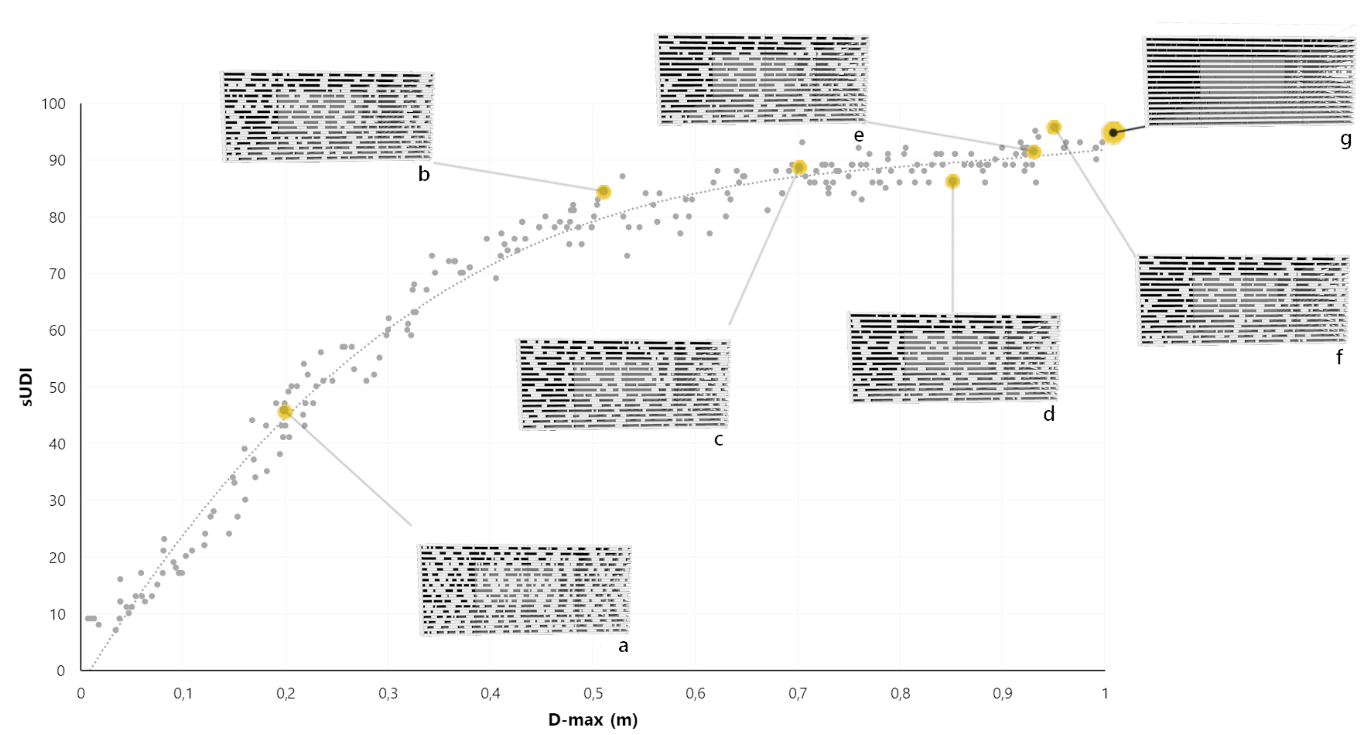
\includegraphics[width=\textwidth]{Images/Evaluation/Ericeira_caadria2018.PNG}
%	\caption{Ericeira Solarium: The scatter plot with the samples obtained during the design of experiments approach. The models a. to g. correspond to the set of examples presented to the architects.}
%	\label{fig:ericeira_doe}
%\end{figure}

\begin{figure}
	\centering
	\includegraphics[width=\textwidth]{Images/Evaluation/Ericeira_2.png}
	\caption{Ericeira Solarium: Representation of the shading panels’ geometric pattern with different sUDI values (from left to right, 7\%, 62\%, 90\%, and 100\%).}
	\label{fig:ericeira_multiple_panels}
\end{figure}

Although this approach did achieve an optimal solution with an 100\% value of sUDI after 200 function evaluations, this approach consists on the consecutive experimentation of multiple designs that are generated randomly and, consequently, does not provide guarantees that optimal solutions will be found. In this case study, we exploited the existing knowledge about the problem to create a more focused design of experiments approach, however it required several manual interventions (e.g., analyse the results, redefine the variables' bounds, select number of evaluations). As a result, we decided to use a more informed and automated approach \cite{Belem2018optimizeddesign}. Because this was a single-objective problem, we followed a simple \ac{SOO} approach (see \cref{ssec:soo}) and we evaluated the performance of 13 different derivative-free optimization algorithms: 5 direct-search, 3 metaheuristics, and 5 model-based. Given the time complexity of each function evaluation, we set a limit of 60 function evaluations per run.

\Cref{table:phase1results} shows the mean best results and the standard deviation of the three runs,  discriminated by algorithm. According to the results, in average, all global model-based algorithms, GPR, RBFCC, and RBFCL, were able to find an optimal solution within the first 30 evaluations of the optimization run. Conversely, the local model-based algorithms, COBYLA and BOBYQA, perform rather poorly in this problem, converging to far from optimal solutions after 29 and 48 function evaluations, respectively. Regarding direct-search algorithms, the global algorithm, DIRECT, was able to find a close to optimal solution (with an \ac{sUDI} value of 98\%) in the last function evaluation. While its local variant, DIRECT-L, and others local direct-search algorithms, PRAXIS and SUBPLEX, fell short of the expected and barely managed to improve over the 80\%. Nevertheless, a simplex-based direct-search algorithm, NMS, performed surprisingly well, having achieved an average result of 89.67\% within the first 15 function evaluations. Finally, although metaheuristics performed better than most local model-based and direct-search algorithms, they seem to stagnate in design solutions with sUDI values below the 88\%, after 30 function evaluations.

%http://papers.cumincad.org/data/works/att/caadria2018\_278.pdf
\begin{table}[htbp]
	\centering
	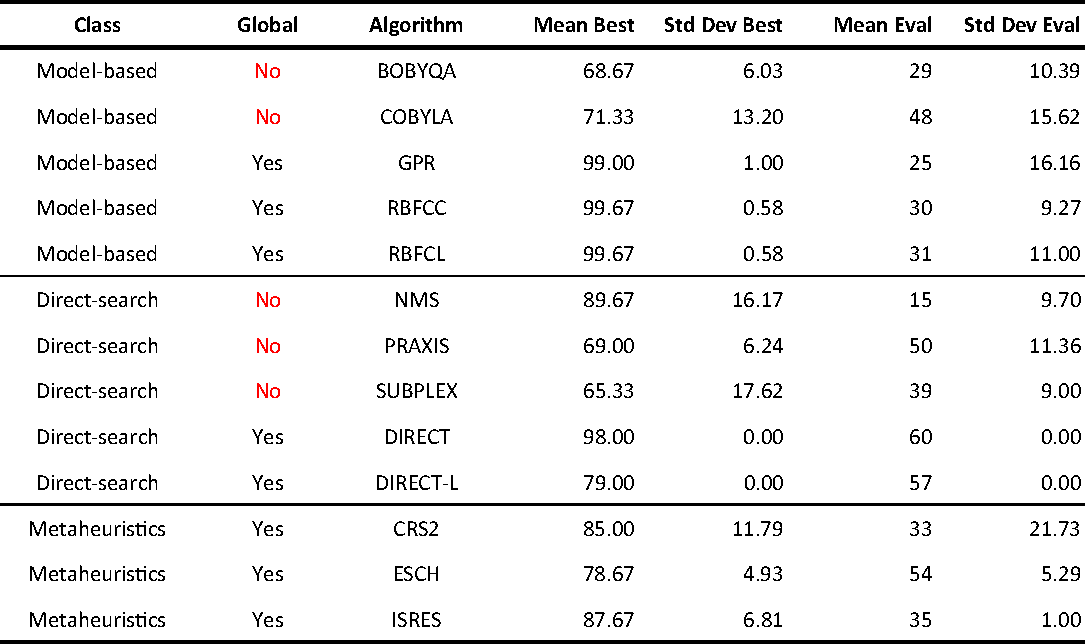
\includegraphics[width=0.8\textwidth]{tables_and_code/Ericeira_phase1_stats_v1.pdf}
	\caption[Ericeira Solarium: Table with best results and necessary evaluations per algorithm]{Ericeira Solarium: Table with the best results of daylight conditions (measured in \ac{sUDI}) per algorithm. Results are averaged over 3 runs, each with 60 evaluations. The table also depicts the average number of necessary evaluations to achieve best results.}
	\label{table:phase1results}
\end{table}

\Cref{fig:phase1results} shows the average performance per algorithm class, also separating them in local or global algorithms. Overall, local algorithms seem to perform worse than all other algorithms, with local direct-search and model-based algorithms stagnating towards design solutions with sUDI values below 75\% and 70\%, respectively. Contrastingly, global algorithms were able to find design solutions with values of sUDI larger than 80\%. Despite the better initial performance of metaheuristics for the first 20 evaluations, global direct-search methods quickly surpassed them, achieving close to optimal solutions with \ac{sUDI} values of 90\%. Global model-based algorithms were the best performing algorithms. 

\begin{figure}[htbp]
	\centering
	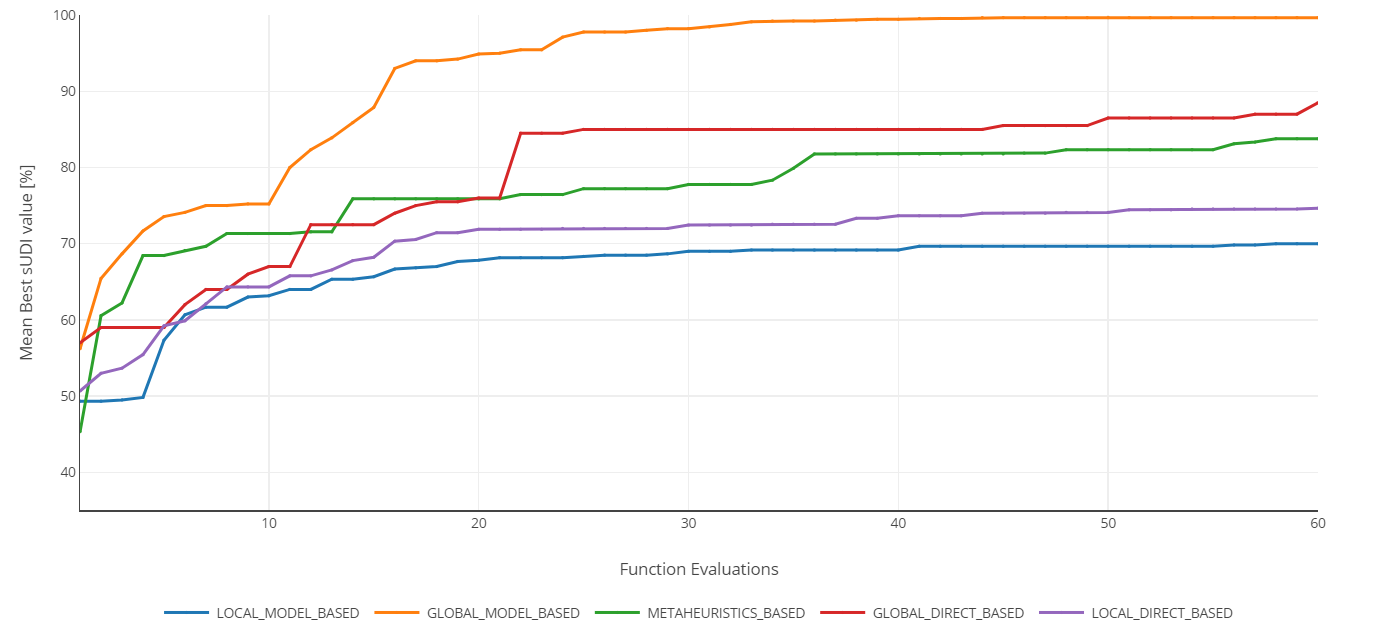
\includegraphics[width=1\textwidth]{Images/Evaluation/Ericeira_results_ph1_per_class.PNG}
	\caption[Ericeira Solarium: Average best results of daylight conditions (measured in \ac{sUDI}) per algorithm's class]{Ericeira Solarium: Average best results of daylight conditions (measured in \ac{sUDI}) per algorithm, as a function of the number of evaluations.}
	\label{fig:phase1results}
\end{figure}

Given the bad performance of local algorithms, we decided to assess their performance when submitted to different initial solutions. Notwithstanding their ability to quickly converge to locally optimal solutions, the quality of the found solutions highly depends on the initial one. To assess the impact of the initial solution in the performance of the algorithms, we submitted them to two different solutions: a bad one with a 7\% value of \ac{sUDI}, and a mild one with a 78\% value of \ac{sUDI}. Moreover, we decided to further constrain the number of function evaluations to 15, thus emulating an ideal scenario, where users lack knowledge about different optimization algorithms, and, as a consequence, opt for testing several algorithms. Ideally, this test would allow them to infer the most promising algorithm and obtain a reasonable solution to hot-start other algorithms and, potentially, improve the overall optimization time.

\Cref{fig:phase2results} presents the mean best daylight conditions found by each local optimization algorithm. As expected no local algorithm was able to obtain a good solution when provided with a bad starting solution. On the one hand, when provided with a mild initial design, both COBYLA and NMS found the best designs achieving a \ac{sUDI} value of 99\%. On the contrary, PRAXIS found the worse, and showed no relevant improvement over the initial design in terms of daylight illuminance. Nevertheless, it initially managed to outperform other methods, achieving values of \ac{sUDI} of 80\%. After the eighth evaluation, COBYLA and NMS quickly converged to near optimal designs, with \ac{sUDI} values of 99\% and 98\%, respectively. BOBYQA and SUBPLEX struggled to improve from the initial design.

On the other hand, when provided with a bad initial design, the best daylight illuminance result has a \ac{sUDI} value of 15\% and was found by NMS after the ninth evaluation. NMS, COBYLA, and SUBPLEX exhibit similar performances, stagnating in a design with a \ac{sUDI} value of 11\% after 3 evaluations, with NMS being able to further improve the design after 5 evaluations. PRAXIS exhibits the worst performance among all methods, showing no significant improvements throughout the whole optimization process.

\begin{figure}[htbp]
	\centering
	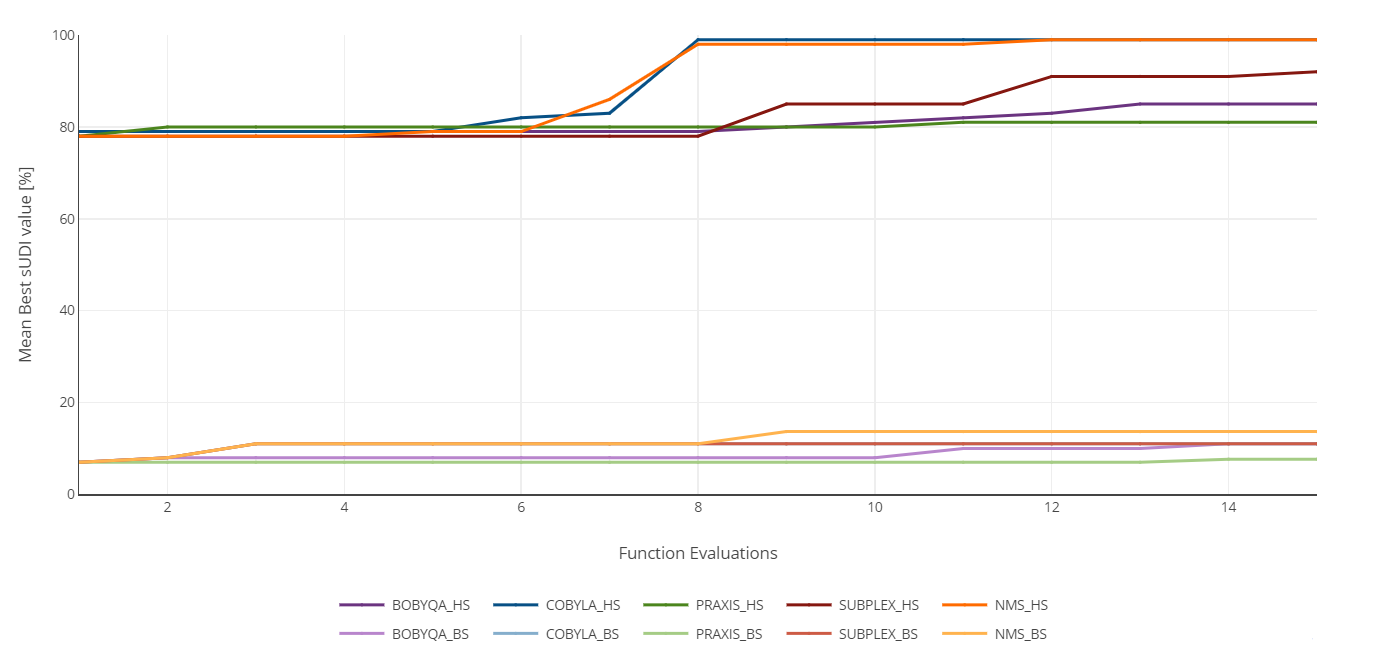
\includegraphics[width=\textwidth]{Images/Evaluation/Ericeira_results_ph2.PNG}
	\caption[Ericeira Solarium: Average best results of daylight conditions (measured in \ac{sUDI}) per local algorithm]{Ericeira Solarium: Average best results of daylight conditions (measured in \ac{sUDI} per local algorithm, as a function of the number of function evaluations. Algorithms suffixed with HS are given an initial solution with an sUDI value of 78\%, whilst algorithms suffixed with BS are given an initial solution with an sUDI value of 7\%.}
	\label{fig:phase2results}
\end{figure}


% #############################################################################
\subsection{Space Frame Optimization}

Besides the real-world case study, we decided to focus in \ac{MOO} problems ~\cite{Belem2019MOO}. Given the interest of architects in performing structural analysis \cite{Cichocka2017SURVEY}, we created an artificial case study that optimizes both structural and irregularity aspects of an arc-shaped space frame. To instil irregularities in the space frame, we introduced three attractors to cause a deformation in the shape of the truss. In this case, the parameters are the fixed-radius cylindrical coordinates of the three attractors and the goal is to optimize the structural aspect, measured in terms of the maximum displacement, and the irregularity aspect, measured in terms of the sum of the Euclidean distances between the three attractors. \Cref{fig:spaceframe} illustrates three examples of the space frame structure. 

\begin{figure}[htbp]
	\centering
	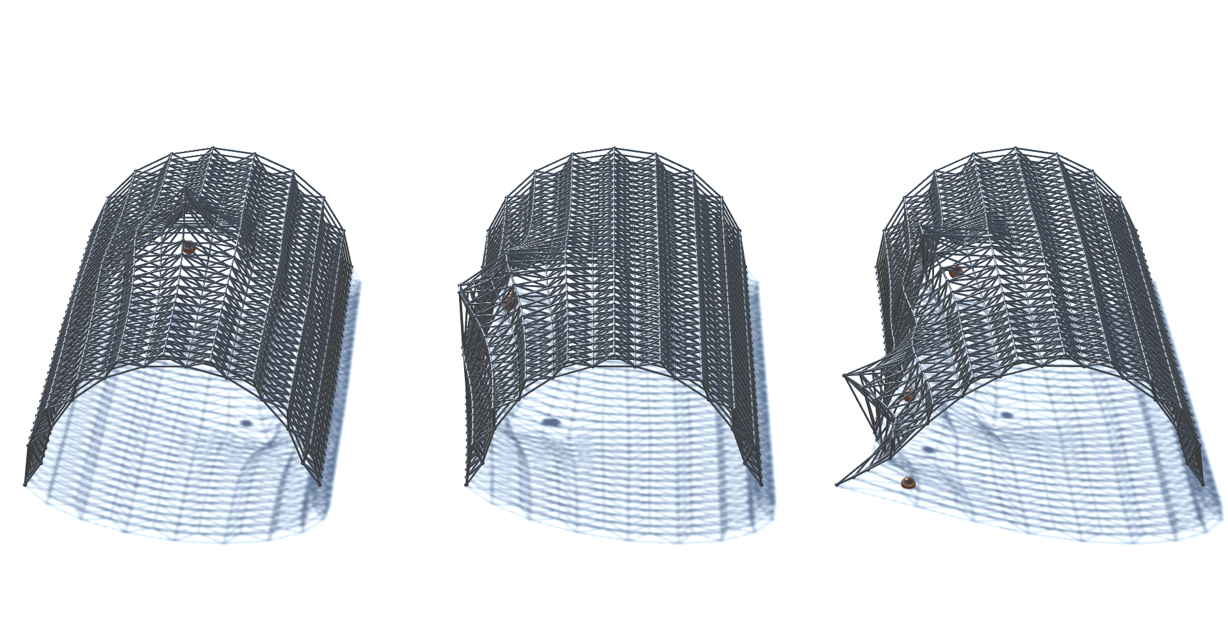
\includegraphics[width=1\textwidth]{Images/Evaluation/truss-kat.png}
	\caption[Space Frame: Representation of three space frame design variants]{Space Frame: Representation of three design variations of the arc-shaped space frame, with copper balls representing the three attractors.}
	\label{fig:spaceframe}
\end{figure}

We evaluated 


\subsection{Black Pavilion: Skylights Optimization}

- INVOLVE OPTIMIZAÇÃO LUMINICA E DE CUSTO.


\subsection{Other cases...}

- Adaptive Façades: Thermal